%%%%%%%%%%%%%%%%%%%%%%%%%%%%%%%%%%%%%%%%%%%%%%%%%%%%%%%%%%%%%%%%%%%%%%%%%%%%%%%%%%%%%%%%%%%%%%%%%%%%%%%%%%%%%%%%%%%%%%%%%%%%%%%%%%%%%%%%%%%%%%%%%%%%%%%%%%%
% This is just an example/guide for you to refer to when submitting manuscripts to Frontiers, it is not mandatory to use Frontiers .cls files nor frontiers.tex  %
% This will only generate the Manuscript, the final article will be typeset by Frontiers after acceptance.   
%                                              %
%                                                                                                                                                         %
% When submitting your files, remember to upload this *tex file, the pdf generated with it, the *bib file (if bibliography is not within the *tex) and all the figures.
%%%%%%%%%%%%%%%%%%%%%%%%%%%%%%%%%%%%%%%%%%%%%%%%%%%%%%%%%%%%%%%%%%%%%%%%%%%%%%%%%%%%%%%%%%%%%%%%%%%%%%%%%%%%%%%%%%%%%%%%%%%%%%%%%%%%%%%%%%%%%%%%%%%%%%%%%%%

%%% Version 3.4 Generated 2018/06/15 %%%
%%% You will need to have the following packages installed: datetime, fmtcount, etoolbox, fcprefix, which are normally inlcuded in WinEdt. %%%
%%% In http://www.ctan.org/ you can find the packages and how to install them, if necessary. %%%
%%%  NB logo1.jpg is required in the path in order to correctly compile front page header %%%

\documentclass[utf8]{frontiersSCNS} % for Science, Engineering and Humanities and Social Sciences articles
\usepackage{url,hyperref,lineno,listings,microtype,subcaption}
\usepackage[onehalfspacing]{setspace}

% Automatic formatting of SI units
\usepackage[binary-units,separate-uncertainty=true]{siunitx}

% Required for 'straight' quotes in code listings
\usepackage[T1]{fontenc}

% Visible TODO notes
\newcommand{\todo}[1]{\textbf{\textsc{\textcolor{red}{(TODO: #1)}}}}

% Configure code listings
\lstset{language=C++,showstringspaces=false,basicstyle=\tiny,upquote=true,identifierstyle=\ttfamily\color{black}}
\lstset{language=Python,showstringspaces=false,basicstyle=\tiny,upquote=true,identifierstyle=\ttfamily\color{black}}

\linenumbers


\def\keyFont{\fontsize{8}{11}\helveticabold }
\def\firstAuthorLast{Knight and Nowotny} %use et al only if is more than 1 author
\def\Authors{James C Knight\,$^{1,*}$, Anton Komissarov, Thomas Nowotny\,$^{1}$}
\def\Address{$^{1}$Centre for Computational Neuroscience and Robotics, School of Engineering and Informatics, University of Sussex, Brighton, United Kingdom }
\def\corrAuthor{James C Knight}
\def\corrEmail{J.C.Knight@sussex.ac.uk}

\begin{document}
\onecolumn
\firstpage{1}

\title[PyGeNN]{PyGeNN: A Python library for GPU-enhanced neural networks} 

\author[\firstAuthorLast ]{\Authors} %This field will be automatically populated
\address{} %This field will be automatically populated
\correspondance{} %This field will be automatically populated

\extraAuth{}% If there are more than 1 corresponding author, comment this line and uncomment the next one.
%\extraAuth{corresponding Author2 \\ Laboratory X2, Institute X2, Department X2, Organization X2, Street X2, City X2 , State XX2 (only USA, Canada and Australia), Zip Code2, X2 Country X2, email2@uni2.edu}


\maketitle


\begin{abstract}

%%% Leave the Abstract empty if your article does not require one, please see the Summary Table for full details.
\section{}
For full guidelines regarding your manuscript please refer to \href{http://www.frontiersin.org/about/AuthorGuidelines}{Author Guidelines}.

As a primary goal, the abstract should render the general significance and conceptual advance of the work clearly accessible to a broad readership. References should not be cited in the abstract. Leave the Abstract empty if your article does not require one, please see \href{http://www.frontiersin.org/about/AuthorGuidelines#SummaryTable}{Summary Table} for details according to article type. 

\tiny
 \keyFont{ \section{Keywords:} keyword, keyword, keyword, keyword, keyword, keyword, keyword, keyword} %All article types: you may provide up to 8 keywords; at least 5 are mandatory.
\end{abstract}

\section{Introduction}
A wide range of spiking neural network~(SNN) simulators are available, each with their own niche. 
NEST~\citep{Gewaltig2007} is widely used for large-scale point neuron simulations on distributed computing systems; NEURON~\citep{carnevale2006neuron} and Arbor~\citep{Akar2019} specialise in the simulation of complex multi-compartmental models; and CARLsim~\citep{Chou2018} and GeNN~\citep{Yavuz2016} use Graphics Processing Units~(GPUs) to accelerate point neuron models.
For performance reasons, many of these simulators are written in C++ and, especially amongst the older simulators, users describe their models either using a Domain-Specific Language~(DSL) or directly in C++.
For programming language purists, a DSL may be an elegant way of describing an SNN network model and, for simulator developers, not having to add bindings to another language is convenient.
However, both choices act as a barrier to potential users.
Therefore, with both the computational neuroscience and machine learning communities gradually coalescing towards a Python-based ecosystem with a wealth of mature libraries for scientific computing~\citep{Hunter2007,VanDerWalt2011,Millman2011}, exposing spiking neural network simulators to Python seems a pragmatic choice.
NEST~\citep{Eppler2009}, Neuron~\citep{Hines2009} and CARLsim~\citep{Balaji2020} have all taken this route and now offer a Python interface.
Furthermore, newer simulators such as Arbor and Brian2~\citep{Stimberg2019} have been designed from the ground up with a Python interface.

While we have recently demonstrated some very competitive performance results~\citep{Knight2018,Knight2020} using our GeNN simulator~(Yavuz2016), it has not been usable directly from Python.
GeNN can already be used as a backend for the Python-based Brian2 simulator~\citep{Stimberg2019} but, while Brian2GeNN~\citep{Stimberg2020} allows Brian2 users to harness the performance benefits GeNN provides, it is not possible to expose all of GeNN's unique features to Python through the Brian2 API.
Specifically, GeNN not only allows users to easily define their own neuron and synapse models but, also `snippets' for offloading the potentially costly initialisation of model parameters and connectivity onto the GPU.
Additionally, GeNN  provides a lot of freedom for users to integrate their own code into the simulation loop.
In this paper we describe the implementation of PyGeNN -- a Python package which aims to expose the full range of GeNN functionality with minimal performance overheads.
We then demonstrate this performance using two large-scale models from the literature.

\section{Materials and Methods}
\subsection{GeNN}
\label{sec:methods/genn}
GeNN~\citep{Yavuz2016} is a library for generating CUDA code for the simulation of spiking neural network models.
GeNN handles much of the complexity of using CUDA directly as well as automatically performing device-specific optimizations so as to to maximize performance.

GeNN consists of a main library -- implementing the API used to define models as well as the generic parts of the code generator -- and an additional library for each backend (currently there is a reference C++ backend for generating CPU code and a CUDA backend. An OpenCL backend is under development).
Users describe their model by implementing a \lstinline{modelDefinition} function within a C++ file. For example, a model consisting of 4 Izhikevich neurons with heterogeneous parameters, driven be a constant input current might be defined as follows:
%
\begin{lstlisting}[language=C++]
void modelDefinition(ModelSpec &model)
{
    model.setDT(0.1);
    model.setName("izhikevich");
    
    NeuronModels::IzhikevichVariable::VarValues popInit(
        -65.0, -20.0, uninitialisedVar(), uninitialisedVar(),
        uninitialisedVar(), uninitialisedVar());
    
    model.addNeuronPopulation<NeuronModels::IzhikevichVariable>(
        "Pop", 4, {}, popInit);
        
    CurrentSourceModels::DC::ParamValues csParams(10.0);

    model.addCurrentSource<CurrentSourceModels::DC>(
        "CS", "Neurons", csParams, {});
}
\end{lstlisting}
%
The \emph{genn-buildmodel} command line tool is then used to compile this file; link it against the main GeNN library and the desired backend library; and finally run the resultant executable to generate the source code required to build a simulation dynamic library (a .dll file on Windows or a .so file on Linux and Mac).
This dynamic library can then either be statically linked against a simulation loop provided by the user or dynamically loaded by the users simulation code.
To demonstrate this latter approach, this example uses the \lstinline{SharedLibraryModel} helper class supplied with GeNN to dynamically loads the previously defined model, initialise the heterogenous neuron parameters and print each neuron's membrane voltage every timestep: 
%
\begin{lstlisting}[language=C++]
#include "sharedLibraryModel.h"

int main()
{
    SharedLibraryModel<float> model("./", "izhikevich");
    model.allocateMem();
    model.initialize();
    float *aPop = model.getScalar<float>("a");
    float *bPop = model.getScalar<float>("b");
    float *cPop = model.getScalar<float>("c");
    float *dPop = model.getScalar<float>("d");
    aPop[0] = 0.02; bPop[0] = 0.2;  cPop[0] = -65.0;    dPop[0] = 8.0;  // RS
    aPop[1] = 0.1;  bPop[1] = 0.2;  cPop[1] = -65.0;    dPop[1] = 2.0;  // FS
    aPop[2] = 0.02; bPop[2] = 0.2;  cPop[2] = -50.0;    dPop[2] = 2.0;  // CH
    aPop[3] = 0.02; bPop[3] = 0.2;  cPop[3] = -55.0;    dPop[3] = 4.0;  // IB
    model.initializeSparse();

    float *vPop = model.getScalar<float>("VPop");
    while(model.getTime() < 200.0f) {
        model.stepTime();
        model.pullVarFromDevice("Pop", "V");
        printf("%f, %f, %f, %f, %f\n", t, VPop[0], VPop[1], VPop[2], VPop[3]);
    }
    return EXIT_SUCCESS;
}
\end{lstlisting}

\subsection{SWIG}
In order to use GeNN from Python, both the model creation API and the \lstinline{SharedLibraryModel} functionality need to be `wrapped' so they can be called from Python.
While this is possible using the API built into Python itself, a wrapper function would need to be manually implemented for each GeNN function to be exposed which would result in a lot of maintenance overhead.
Instead, we chose to use SWIG~\citep{Beazley1996} to automatically generate wrapper functions and classes. 
SWIG generates Python modules based on special interface files which can directly include C++ code as well as special `directives' which directly control SWIG:
%
\begin{lstlisting}[language=C++]
%module(package="package") package
%include "test.h" 
\end{lstlisting}
%
where the \lstinline{%module} directive sets the name of the generated module and the package it will be located in and the \lstinline{%include} directive parses and automatically generates wrapper functions for a C++ header file.
We use SWIG in this manner to wrap both the model building and \lstinline{SharedLibraryModel} APIs described in section~\ref{sec:methods/genn}.
However, key parts of GeNN's API such as the \lstinline{ModelSpec::addNeuronPopulation} method employed in section~\ref{sec:methods/genn}, rely on C++ templates which do not have an equivalent in Python.
Instead, valid template instantiations need to be given a unique name in Python using the \lstinline{%template} SWIG directive:
%
\begin{lstlisting}[language=C++]
%template(addNeuronPopulationLIF) ModelSpec::addNeuronPopulation<NeuronModels::LIF>;
\end{lstlisting}
%
Having to manually add these directives whenever a model is added to GeNN would be exactly the sort of maintenance overhead we were trying to avoid by using SWIG.
Instead, when building the Python wrapper, we search the GeNN header files for the macros used to declare models in C++ and automatically generate SWIG \lstinline{%template} directives.

As previously discussed, a key feature of GeNN is the ease with which it allows users to define their own neuron and synapse models as well as `snippets' defining how variables and connectivity should be initialised.
Beneath the syntactic sugar described in our previous work~\citep{Knight2018}, new models can be defined in C++ by defining a new class derived from, for example, the \lstinline{NeuronModels::Base} class.
The ability to extend this system to Python was a key requirement of PyGeNN and, by using SWIG `directors', C++ classes can be made inheritable from Python using a single SWIG directive:
%
\begin{lstlisting}[language=C++]
%feature("director") NeuronModels::Base; 
\end{lstlisting}
%
\subsection{PyGeNN}
While GeNN \emph{could} be used from Python via the wrapper generated using the techniques described in the previous section, the resultant code would be unpleasant to use directly.
For example, rather than being able to specify neuron parameters using a native Python data structure such as a list or dictionary, you have to use a wrapped type such as \lstinline{DoubleVector([0.25, 10.0, 0.0, 0.0, 20.0, 2.0, 0.5])}.
To provide a more user-friendly and pythonic interface, we have built PyGeNN on top of the wrapper generated by SWIG.
PyGeNN combines the separate model building and simulation stages of building a GeNN model in C++ into a single API, likely to be more familiar to users of existing Python-based model description languages such as PyNEST~\citep{Eppler2009} or PyNN~\citep{Davison2008}.
This allows PyGeNN to provide a unified dictionary-based API for initialising homogeneous and heterogeneous parameters as shown in this re-implementation of the previous example:
%
\begin{lstlisting}[language=Python]
from pygenn import genn_wrapper, genn_model

model = genn_model.GeNNModel("float", "izhikevich")
model.dT = 0.1

izk_init = {"V": -65.0,
            "U": -20.0,
            "a": [0.02,     0.1,    0.02,   0.02],
            "b": [0.2,      0.2,    0.2,    0.2],
            "c": [-65.0,    -65.0,  -50.0,  -55.0],
            "d": [8.0,      2.0,    2.0,    4.0]}

pop = model.add_neuron_population("Pop", 4, "IzhikevichVariable", {}, izk_init)
model.add_current_source("CS", "DC", "Neurons", {"amp": 10.0}, {})

model.build()
model.load()

v = pop.vars["V"].view
while model.t < 200.0:
    model.step_time()
    model.pull_state_from_device("Neurons")
    print("%t, %f, %f, %f, %f" %(model.t, v[0], v[1], v[2], v[3]))
\end{lstlisting}
%
While the PyGeNN API is more pythonic and, hopefully, more user-friendly than the C++ interface to GeNN, it still allows the user the same amount of control with respect to defining their own simulation loop.
Additionally, by using SWIG's numpy~\citep{VanDerWalt2011} interface, the host memory allocated by GeNN can be accessed directly from Python using the \lstinline{pop.vars["V"].view} syntax meaning that no potentially additional expensive copying of data is required.
\todo{defining new neuron models}
%
\begin{figure}
    \begin{center}
        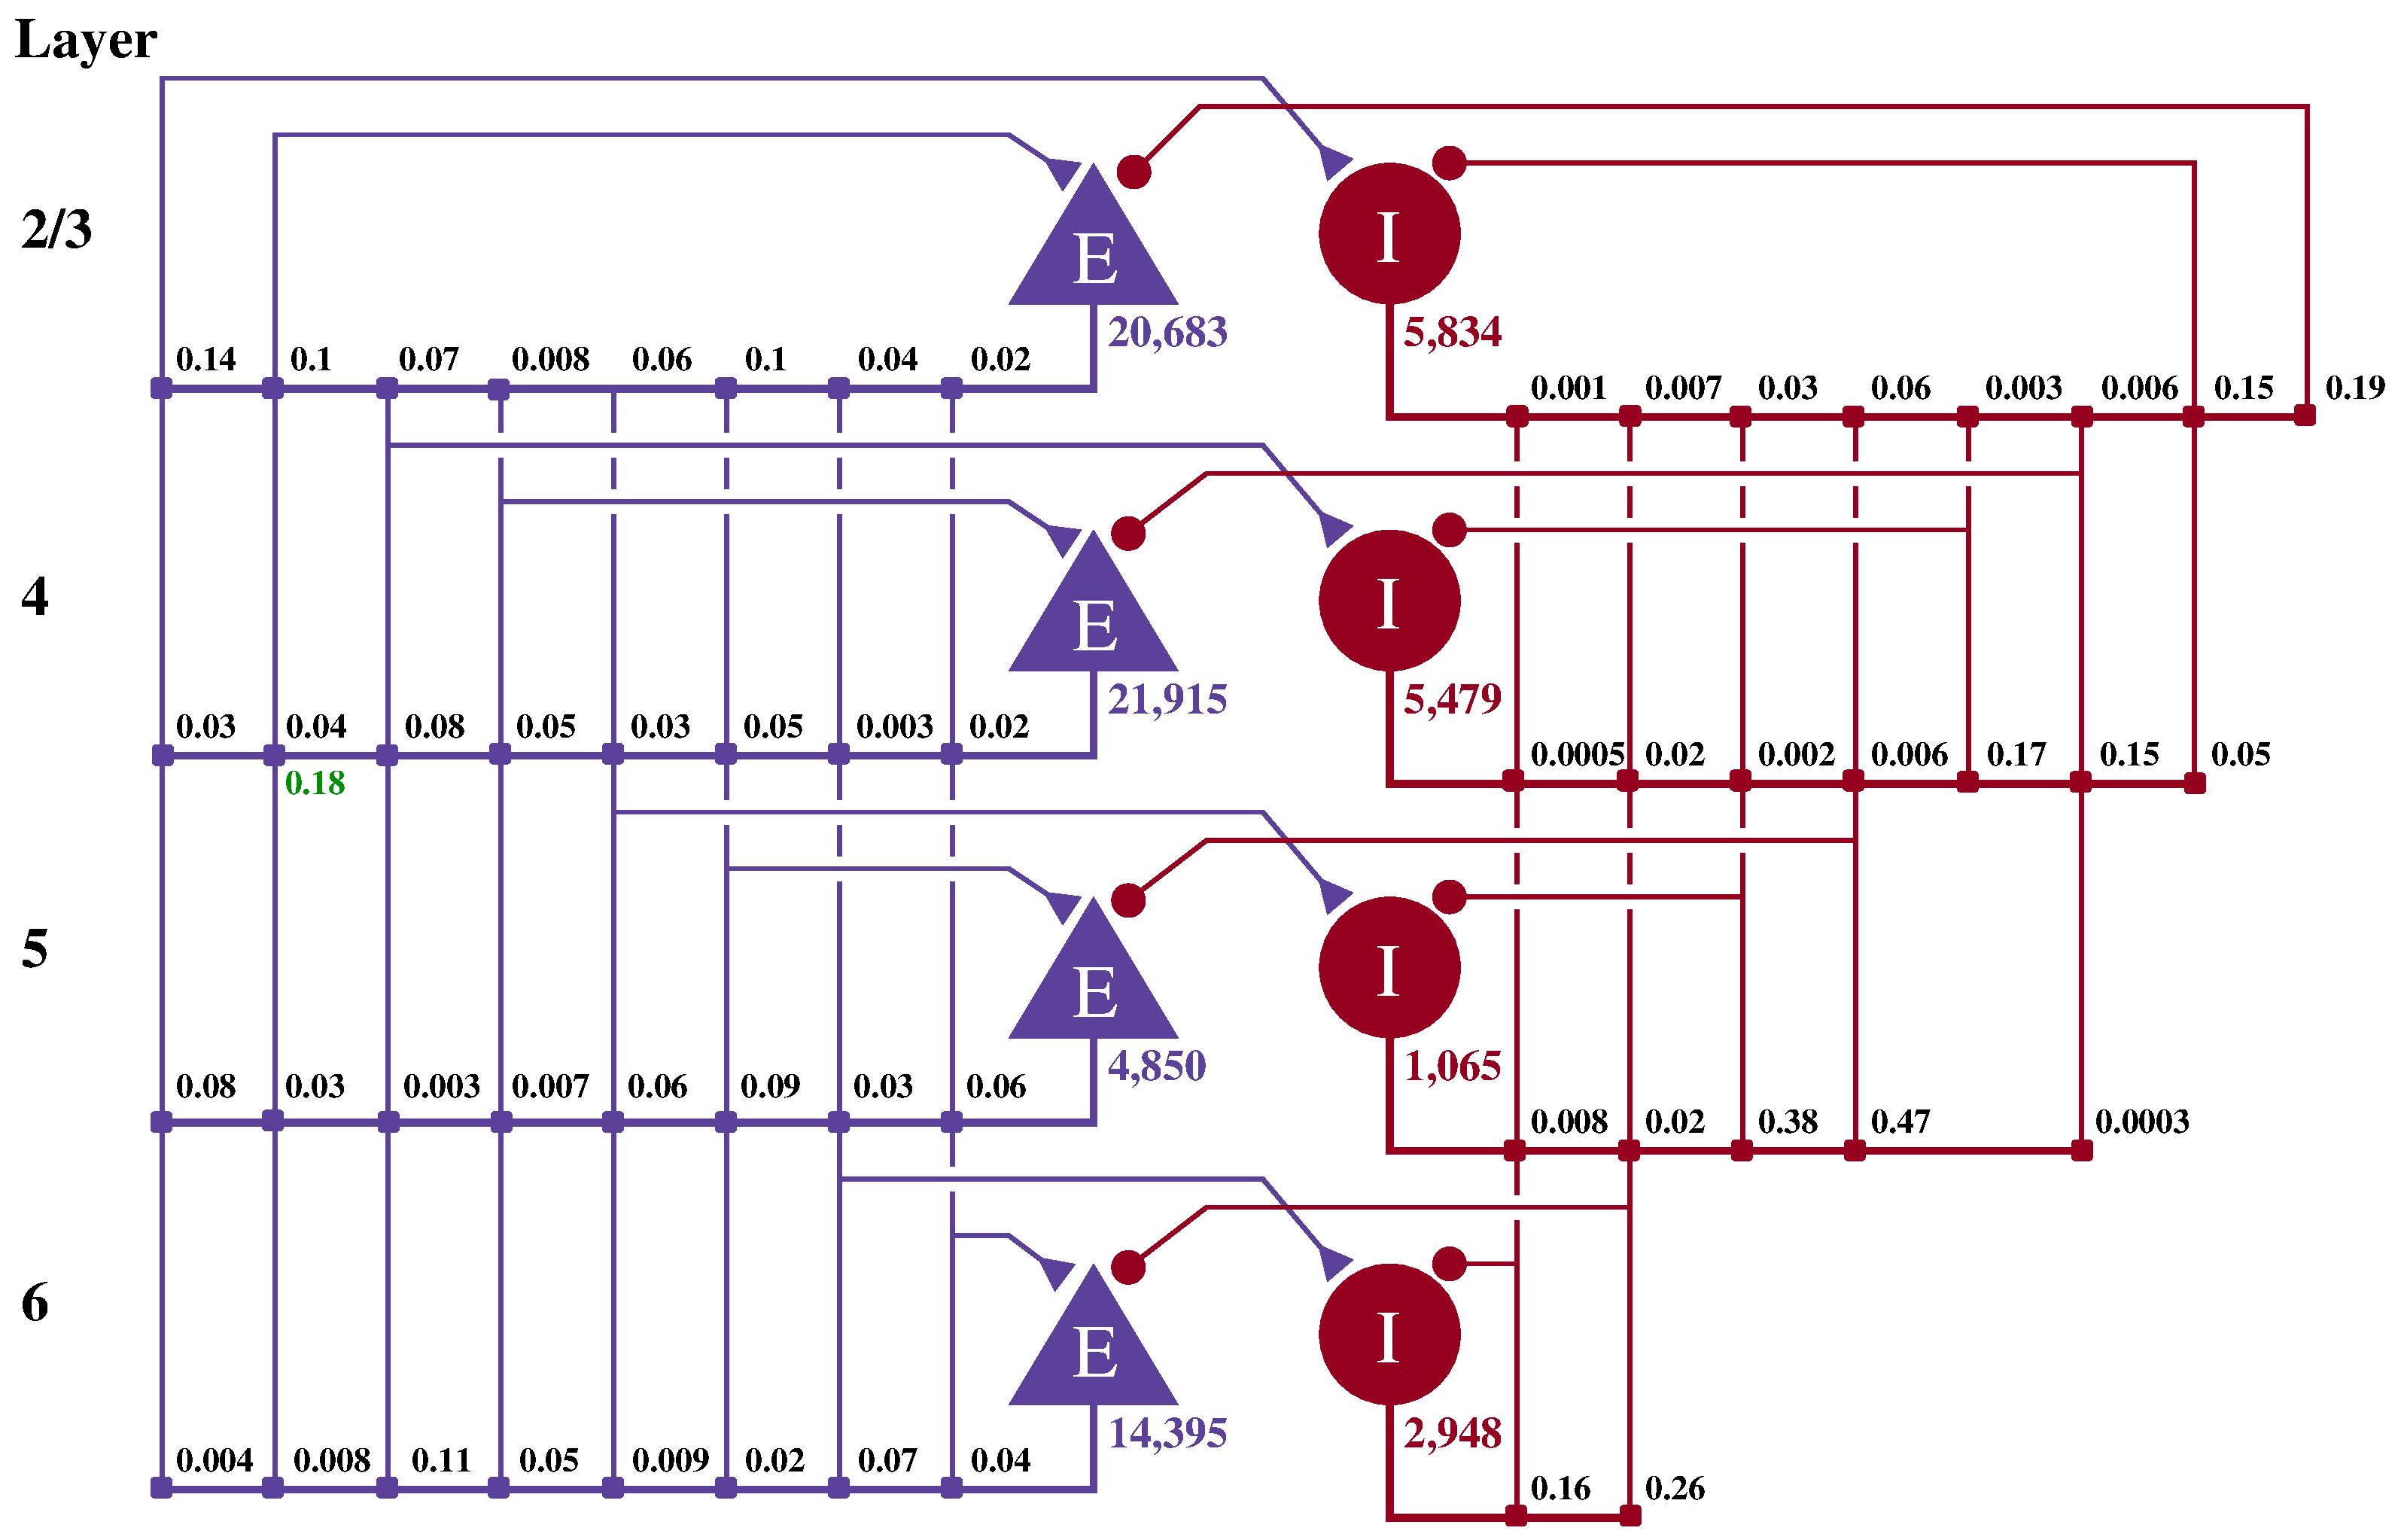
\includegraphics[width=180mm]{figures/potjans_circuit_v2}
    \end{center}
    \caption{Illustration of the microcircuit model.
    Blue triangles represent excitatory populations, red circles represent inhibitory populations and the numbers beneath each symbol shows the number of neurons in each population.
    Connection probabilities are shown in small bold numbers at the appropriate point in the connection matrix.
    All excitatory synaptic weights are normally distributed with a mean of \SI{0.0878}{\nano\ampere} (unless otherwise indicated in green) and a standard deviation of \SI{0.00878}{\nano\ampere}.
    All inhibitory synaptic weights are normally distributed with a mean of \SI{0.3512}{\nano\ampere} and a standard deviation of \SI{0.03512}{\nano\ampere}.}
    \label{fig:potjans_circuit}
\end{figure}
%
\subsection{Spike recording system}
\label{sec:methods/spike_recording}
Internally, GeNN stores the spikes emitted by a neuron population during one simulation timestep in an array containing the indices of the neurons that spiked alongside a counter of how many spikes have been emitted.
Previously, recording spikes in GeNN was very similar to the recording of voltages shown in the previous example code -- the array of neuron indices was simply copied from the GPU to the CPU every timestep.
However, especially when simulating models with a small simulation timestep, such frequent synchronization between the CPU and GPU is costly.
Furthermore, biological neurons typically spike at a low rate (in the cortex, the average firing rate is only around \SI{3}{\hertz}~\citep{Buzsaki2014}) meaning that the amount of spike data transferred every timestep would typically be small.
To address both of these sources of inefficiency, we have added a new data structure to GeNN which stores spike data for many timesteps on device.
To reduce the memory required for this data structure and to make its size independent of neural activity, the spikes emitted by a population of $N$ neurons in a single simulation timestep are stored in a $N\si{\bit}$ bitfield where a `1' represents a spike and a `0' the absence of one.
Spiking data over multiple timesteps is then represented by bitfields stored in a circular buffer.
Using this approach, even the spiking output of relatively large models, running for many timesteps can be stored in a small amount of memory.
For example, the spiking output of a model with \num{100E3} neurons running for \num{10E3} simulation timesteps, required less than \SI{120}{\mega\byte} -- a small fraction of the memory on a modern GPU.
While efficiently handling spikes stored in a bitfield is a little trickier than working with a list of neuron indices, GeNN provides an efficient C++ helper function for saving the spikes stored in a bitfield to a text file and a numpy-based method for decoding them in PyGeNN. 
%
\begin{figure}
    \begin{center}
        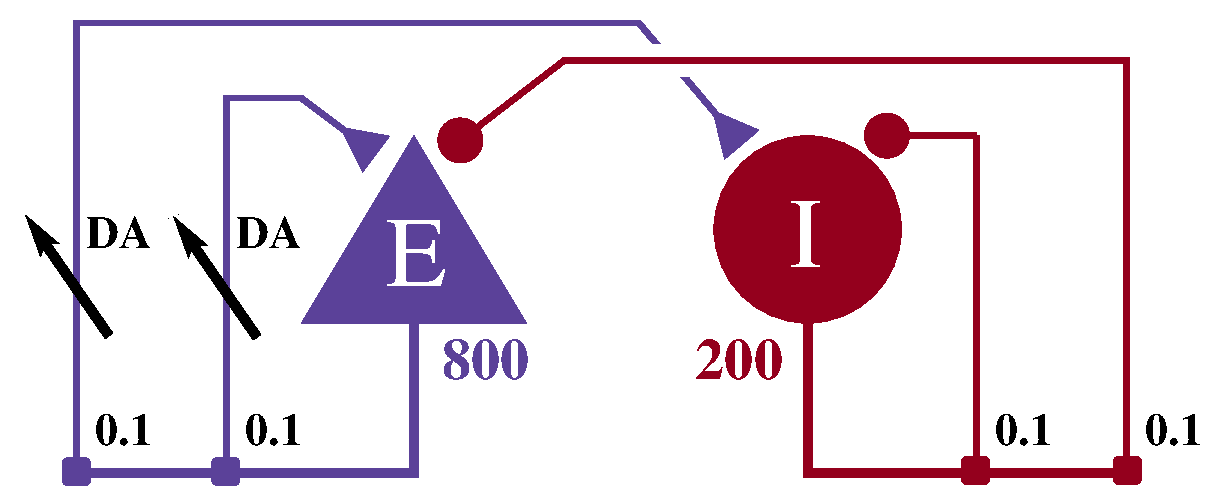
\includegraphics[width=85mm]{figures/circuit2}
    \end{center}
    \caption{Illustration of the balanced random network model.
    The blue triangle represents the excitatory population, the red circle represents the inhibitory population, and the numbers beneath each symbol show the number of neurons in each population.
    Connection probabilities are shown in small bold numbers at the appropriate point in the connection matrix.
    All excitatory synaptic weights are initialised to \SI{0.04561}{\nano\ampere} and all inhibitory synaptic weights are initialised to \SI{0.22805}{\nano\ampere}.}
    \label{fig:balanced_random_circuit}
\end{figure}
%
\subsection{Cortical microcircuit model}
\citet{Potjans2012} developed this model of \SI{1}{\milli\metre\cubed} of early-sensory cortex.
The model consists of \num{77169} neurons, divided into separate populations representing the excitatory and inhibitory population in each of 4 cortical layers~(2/3, 4, 5 and 6).
Neurons in each population are connected randomly with population-specific densities derived from an extensive review of the anatomical literature resulting in a total of approximately \num{0.3E9} synapses. % REWRITE SENTENCE
Within each synaptic projection, all synaptic strengths and transmission delays are normally distributed.
As well as its synaptic input, each neuron in the network also receives an independent Poisson input current, representing input from neighbouring un-modelled cortical regions.
For a full description of the model parameters, please refer to \citet[tables 4 and 5]{Potjans2012} and for a description of the strategies used by GeNN to parallelise the initialisation and subsequent simulation of this network, please refer to \citet[section 2.3]{Knight2018}.
This model requires simulation using a relatively small timestep of \SI{0.1}{\milli\second}, making the overheads of copying spikes from the GPU every timestep particularly significant.

\subsection{Random balanced network HPC benchmark model}
sdasd

\section{Results}
asfgaf

\subsection{Cortical microcircuit model performance}
Figure~\ref{fig:microcircuit_overheads} shows the simulation times for the full-scale microcircuit mode on a representative selection of NVIDIA GPU hardware:
%
\begin{figure}[h!]
    \begin{center}
        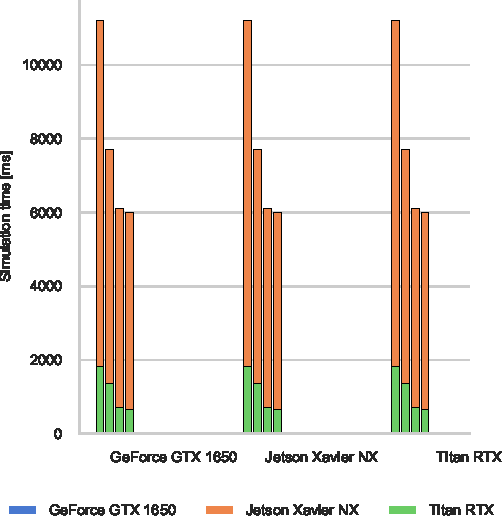
\includegraphics{figures/microcircuit_overheads.pdf}
    \end{center}
    \caption{Simulation times of the microcircuit model running on various GPU hardware for \SI{1}{\second} of biological time.
    `Overhead' refers to time spent in simulation loop but not within CUDA kernels.
    The dotted horizontal line indicates realtime performance}
    \label{fig:microcircuit_overheads}
\end{figure}
%
\begin{figure}[h!]
    \begin{center}
        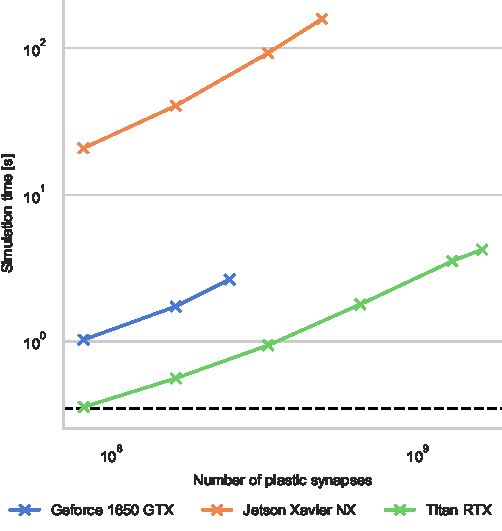
\includegraphics{figures/hpc_benchmark.pdf}
    \end{center}
    \caption{}
    \label{fig:hpc_benchmark}
\end{figure}
%
\begin{itemize}
    \item Jetson Xavier NX -- a low-power embedded system with \SI{8}{\giga\byte} of shared memory.
    \item GeForce GTX 1650 -- a low-end desktop GPU with \SI{4}{\giga\byte} of dedicated memory.
    \item Titan RTX -- a high-end workstation GPU with \SI{24}{\giga\byte} of dedicated memory.
\end{itemize}
%
As one might predict, the Jetson Xavier NX is slower than the two desktop GPUs.
However, considering that it only consumes a maximum of \SI{15}{\watt} compared to \SI{75}{\watt} or \SI{320}{\watt} for the GeForce GTX 1650 and Titan RTX respectively, it still performs impressively.

The time taken to actually simulate the models (`Neuron simulation' and `Synapse simulation') are the same when using Python and C++ as all GeNN optimisation options are exposed to PyGeNN.
However, both the PyGeNN and C++ simulations spend a significant amount of every simulation step copying spike data off the device and storing it in a suitable data structure (`Overhead').
Because Python is an interpreted language, such operations are inherently slower -- this is particularly noticeable on devices with a slower CPU such as the Jetson Xavier NX.
Unlike the desktop GPUs, the Jetson Xavier NX's \SI{8}{\giga\byte} of memory is shared between the GPU and the CPU meaning that data doesn't have to be copied between GPU and CPU memory and can instead by accessed by both.
\todo{run xavier NX without recording and without zero copy}
While, using this shared memory for recording spikes, reduces the overheads associated with copying data off the device, because the GPU and CPU caches are not coherent, caching must be disabled on this memory which reduces the performance of the neuron kernel.
However, when the spike recording system described in section~\ref{sec:methods/spike_recording} is used, spike data is kept in GPU memory until the end of the simulation and this overhead is reduced by around a factor of 10.
This now means that, on the high-end desktop GPU, this simulation now runs faster than real-time -- previously only achievable using a specialised neuromorphic system~\citep{Rhodes2019} and significantly faster than other recently published GPU simulators~\citep{Golosio2020}.

\section{Discussion}
discuss!
\begin{itemize}
    \item PyGeNN as an intermediate layer - PyNN, ML
    \item Cost of C++ - Python calls in models
\end{itemize}

\section*{Conflict of Interest Statement}
The authors declare that the research was conducted in the absence of any commercial or financial relationships that could be construed as a potential conflict of interest.

\section*{Author Contributions}
JK and TN wrote the paper.
TN is the original developer of GeNN.
AK was the original developer of PyGeNN.
JK is currently the primary developer of both GeNN and PyGeNN and was responsible for implementing the spike recording system.
JK performed the experiments and the analysis of the results that are presented in this work.

\section*{Funding}
This work was funded by the EPSRC (Brains on Board project, grant number EP/P006094/1).

\section*{Acknowledgments}
This is a short text to acknowledge the contributions of specific colleagues, institutions, or agencies that aided the efforts of the authors.

\section*{Data Availability Statement}
The datasets [GENERATED/ANALYZED] for this study can be found in the [NAME OF REPOSITORY] [LINK].
% Please see the availability of data guidelines for more information, at https://www.frontiersin.org/about/author-guidelines#AvailabilityofData

\bibliographystyle{frontiersinSCNS_ENG_HUMS} % for Science, Engineering and Humanities and Social Sciences articles, for Humanities and Social Sciences articles please include page numbers in the in-text citations
\bibliography{pygenn}

\end{document}
